%   Filename    : chapter_1.tex 
\chapter{Introduction}
\label{sec:researchdesc}    %labels help you reference sections of your document

\section{Overview of the Current State of Technology}
\label{sec:overview}

The ability to read is a fundamental skill that is necessary for success in many areas of life. Unfortunately, there are many adults in the Philippines who have never learned to read or who have difficulty reading due to various reasons such as illiteracy, limited education, or learning disabilities. These individuals often face significant barriers to employment, education, and social participation, leading to a cycle of poverty and marginalization.

In 2019, the Philippines achieved a literacy rate of 96.5 \% for the segment of the population aged 10 and over according to the PSA’s Functional Literacy, Education and Mass Media Survey (FLEMMS), as reported in an article from Business World entitled, “Literacy rate estimated at 93.8\% among 5 year olds or older — PSA.” Literacy was defined as the ability to read and write “with understanding of simple messages in any language or dialect.” However, the same article notes that this was the same rate observed in 2013, a matter described as alarming by University of Asia and the Pacific Senior Economist Cid L. Terosa, stating that even minimal improvements should be expected especially after six years.

More recently, according to a report published by UNICEF in collaboration with UNESCO and the World Bank, the percentage of 10-year-olds in low- and middle-income countries who are unable to read is as high as 70\%. This figure has likely been affected by school closures brought about by the COVID-19 pandemic. The same report also stated that only 10\% of children in the Philippines were able to read simple text as of March 2022. Alarmingly, a separate report published by the World Bank in 2021 found that the rate of learning poverty - defined as the inability to read simple text by age 10 - in the Philippines was at 90\%. These statistics highlight the urgent need to address the education crisis in the Philippines and the need to further augment the country’s current literacy situation.

To address this problem, we propose the development of an automatic reading miscue detection system called Readable, specifically targeting the Hiligaynon language. Hiligaynon, also known as Ilonggo, is an Austronesian language spoken in the Western Visayas region of the Philippines, particularly in the provinces of Iloilo, Guimaras, Negros Occidental, and Capiz. It is one of the major languages of the Philippines, spoken by millions of people as a first or second language.
Our reading miscue detection system will utilize machine learning techniques including automatic speech recognition (ASR). ASR is a technology that allows computers to automatically recognize and transcribe spoken language, and it has made significant advances in recent years. However, it can still be challenging to achieve high levels of accuracy for some languages and accents, especially those that are underrepresented in ASR training data. By targeting local languages like Hiligaynon and designing our ASR system to work well for these languages, we can help ensure that our reading tutor is accessible and effective for non-reading adults in the Philippines.

While there are some similar applications like Google Read Along available for reading instruction, they may not be accessible or relevant for many non-reading adults in the Philippines due to language barriers or lack of internet connectivity. By targeting local languages like Hiligaynon and utilizing the benefits of natural language processing and machine learning techniques, our automatic reading tutor can provide personalized and effective reading instruction that is accessible and relevant for non-reading adults in the Philippines. By providing accessible, effective, and scalable reading education in Hiligaynon, we hope to improve the lives and prospects of non-reading adults in the Philippines and break the cycle of poverty and illiteracy. Children with strong literacy skills grow more consistently and confidently in their studies, and reading literacy is a crucial gateway to other learning areas such as the humanities, mathematics, and the sciences. By addressing learning poverty and promoting reading literacy, we can help ensure that children in the Philippines have the opportunity to reach their full potential and succeed in their studies.

  
%--- the following example shows how to include a figure in PNG format
\begin{figure}[t]                %-- use [t] to place figure at top, [b] to place at the bottom, [h] for here
   \centering                    %-- use this to center the figure
   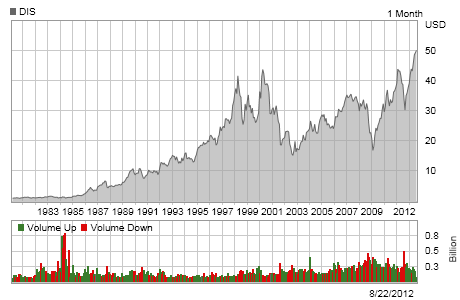
\includegraphics{DisneyChart.png}      %-- include image file named as "disneychart.png" 
   \caption{This is the figure's caption -- Disney stock chart.
   	Captions should fully describe the figure in a concise manner  such that there is not need to refer to the text when figuring out the graphic.}
    \label{fig:disneystock}
\end{figure}


Some notes on citing references.   
When using APA format, the author-date method of citation is  followed.   
This means that the author's last name and the year of publication for the source should  appear in the text, and a complete reference should appear in the reference list.

% Examples:
%     	Smith (1970) compared reaction times . . .
%     	In a recent study of reaction times (Smith, 1970), . . .   
%     	In 1970, Smith compared reaction times . . .
%	    Smith, et al., (1970) compared reaction times . . .
%     	In a recent study of reaction times (Smith, et al., 1970), . .
%     	In 1970, Smith, et al., compared reaction times . . .

Here are some examples on how to do the referencing (note author's name and years are different from commented examples).  
For APA citation details, refer to \url{http://www.ctan.org/tex-archive/biblio/bibtex/contrib/apacite/}. 

\begin{itemize}
 \item \citeA{kartch:2000:ERA} compared reaction times...
 \item In a recent study of reaction times \cite{kartch:2000:ERA}...
 \item In \citeyearNP{kartch:2000:ERA}, \citeauthor{kartch:2000:ERA} compared reaction times...
 \item \shortciteA{fedkiw:2001:VSO} compared reaction times... 
 \item In a recent study of reaction times \cite{fedkiw:2001:VSO}...
 \item In \citeyearNP{fedkiw:2001:VSO}, \shortciteauthor{fedkiw:2001:VSO}, compared reaction times...
\end{itemize}

The following are references from journal articles \cite{Park:2006:DSI, Pellacini:2005:LAH, sako:2001:SSB}.
 Here's an MS thesis document \cite{yee:2000:SSA}, and this is from PhD dissertation \cite{kartch:2000:ERA}. 
 For a book, reference is given as  \cite{parke:1996:CFA}. 
 Proceedings from a conference samples are \cite{Jobs95, fedkiw:2001:VSO, levoy:2000:TDM}.  
 The sample bibliography file named \textbf{myreferences.bib} is from the SIGGRAPH \LaTeX{}  template.  
 You can use a text editor to view the contents of the bib file.  
 It is your task to create your own bibliography file.  
 For those who downloaded papers from ACM or IEEE sites, there is a BibTeX link that you can click; thereafter, you just simply need to copy and paste the BibTeX entry into your own bibliography file.

The following shows how to include a program source code (or algorithm).  
The verbatim environment, as the name suggests, outputs text (including white spaces) as is...

\begin{verbatim}
               #include <stdio.h>
               main()
               {
                    printf("Hello world!\n");
               }
\end{verbatim}

\section{Problem Statement}
\textcolor{red}{DO NOT FORGET to write the statement of the research problem here, i.e., before the Research Objectives.}

A problem statement is your research problem written explicitly.  
The problem statement should do four things: 
\begin{enumerate}
	\item Specify and describe the problem (with appropriate citations) 
	\item  Provide evidence of the problem’s existence  
	\item Explain the consequences of NOT solving the problem  
	\item 	Identify what is not known about the problem that should be known.
\end{enumerate}


\section{Research Objectives}
\label{sec:researchobjectives}

\subsection{General Objective}
\label{sec:generalobjective}

The aim of this project is to develop a reading miscue detection system that would determine the acceptability of an input speech relative to a reference speech pattern.

\subsection{Specific Objectives}
\label{sec:specificobjectives}

%
%  \begin{comment} ... \end{comment} is used for multiple lines of comment
%

\begin{comment}
% IPR acknowledgement: the following sentences and examples are from Ethel Ong's slides 
%     on Research Objectives
How to formulate your research objectives:
1. Identify what research steps do you need to perform to achieve your general objective.
2. Identify the questions that must be answered for you to achieve your general objective.
    Thereafter, convert these questions into action statements

Example #1:

Research Question:
  What are the general features of a web-based learning environment?

Specific Objective:
   To review existing web-based learning environment that teaches language learning for children


Example #2:

Research Question:
   How will you represent commonsense knowledge for use by computer systems?

Specific Objective:
   To identify knowledge representation approaches used by existing story generation systems

Example #3:
Research Question:
   What types of storytelling knowledge are needed to generate stories?

Specific Objective:
    To identify the different types of storytelling knowledge used in generating stories

Example #4:
Research Question:
    What machine learning approaches will you utilize?

Specific Objective:
    To determine existing machine learning algorithms [that can be used in training the computer system to detect cyberbullying cases] 

Example #5: Research Question:
    How will your research output be evaluated?

Specific Objective:
    To define evaluation metrics for validating the accuracy of the translation

\end{comment}

%
%  The following are example specific objectives; replace them with your own 
%
Specifically, the project targets to:
\begin{enumerate}
   \item Train and model a DNN-based acoustic model for Hiligaynon.
   \item Use the developed acoustic model to derive phonemic transcriptions of the input speeches/audio.
   \item Determine the acceptability of a user's speech input, given a set of predetermined words to read, in terms of its deviation from reference transcriptions via forced alignment; judging is based on a set threshold score.
\end{enumerate}


\section{Scope and Limitations of the Research}
\label{sec:scopelimitations}

The system is specific to the Hiligaynon language. The words used in the audio data are limited to 2-3 syllable Hiligaynon words from the book “Hiligaynon Lessons” by Cecille L. Motus. Deviations are only measured word-by-word. In terms of the toolkit, the system is limited by the features offered by Kaldi - an open source speech recognition toolkit for speech recognition and signal processing.

\begin{comment}

%
% IPR acknowledgement: the sentences inside this comment are from Ethel Ong's slides on Scope and Limitations of the Research
%
Generally, one paragraph should be allotted for each of your research objectives.

Each paragraph contains a brief overview of the concept/theory and the purpose of doing the associated objective.

Each paragraph also includes a description of the scope/limitation of your study.

* Please refer to the slides for examples.

\end{comment}


\section{Significance of the Research}
\label{sec:significance}

This project aims to take one step towards developing a solution for improving the reading skill of Filipinos, particularly non reading adults. The authors also aim to contribute to the growing efforts of including Philippine local languages, specifically, Hiligaynon in literatures related to speech processing, particularly those relevant to the development of automated reading tutors.

